
\section{Design}
\label{cp6:design}


% To understand how a tool embedding a semantic-based technique might impact a developer's work,
% we are guided by three main factors.


To design our experiment, we consider three main aspects that assist us examine how a tool that embeds a semantic-based technique might impact a developer's work.



\subsubsection{Requirements}



To be helpful, a tool must direct a developer's attention to \textit{prominent} text that assist them complete a task~\cite{Robillard2015}. If we can gather data about the text in an artifact considered by humans as relevant to the task at hand, we should be able to assess whether the text automatically identified by the tool is similar to the text manually identified. 


In case the text is not similar,
there is a chance that the tool directed a developer to the wrong information, or that 
the tool actually found complementary information that humans missed, which might impact the \textit{correctness} of a task. Therefore, our design must be able to compare the correctness of solutions submitted by participants who perform a task using our envisioned tool against that of developers who attempted the same tasks without tool support, i.e., a control group.


Regardless of how correct participants' solutions are, there is a chance that the text shown by the tool is not \textit{useful}---either because it is not relevant for the task at hand or because it is unsurprising, i.e., the information is ``common-knowledge'' to most developers~\cite{cwalina2008, Robillard2015}. Hence, a successful evaluation would 
ideally
gather qualitative data on the usefulness of the text identified by the tool. 



\subsubsection{Experiment}




Figure~\ref{fig:tool-experiment-procedures} presents an experiment that allows us to address the aforementioned requirements. In this experiment, 24 participants with software development background each attempted a
\textit{manual task} and \textit{tool-assisted task} randomly drawn from a list of well-known Python programming tasks.
Alongside the solution submitted for each task, we use the manual task to collect what text participants deemed relevant to the task performed.
In turn, in the tool-assisted task, we also gathered input on the usefulness of the highlights show. 
This design allow us to:




\begin{itemize}
    \item assess the correctness of the tasks performed \textit{with} or \textit{without} tool support;
    \item compare  the text that participants deemed relevant to the text automatically identified
    and shown in the tool-assisted task, and;
    \item discuss the usefulness of the automatically identified text according to the feedback provided by the participants.
\end{itemize}
 





\begin{figure}
\centering
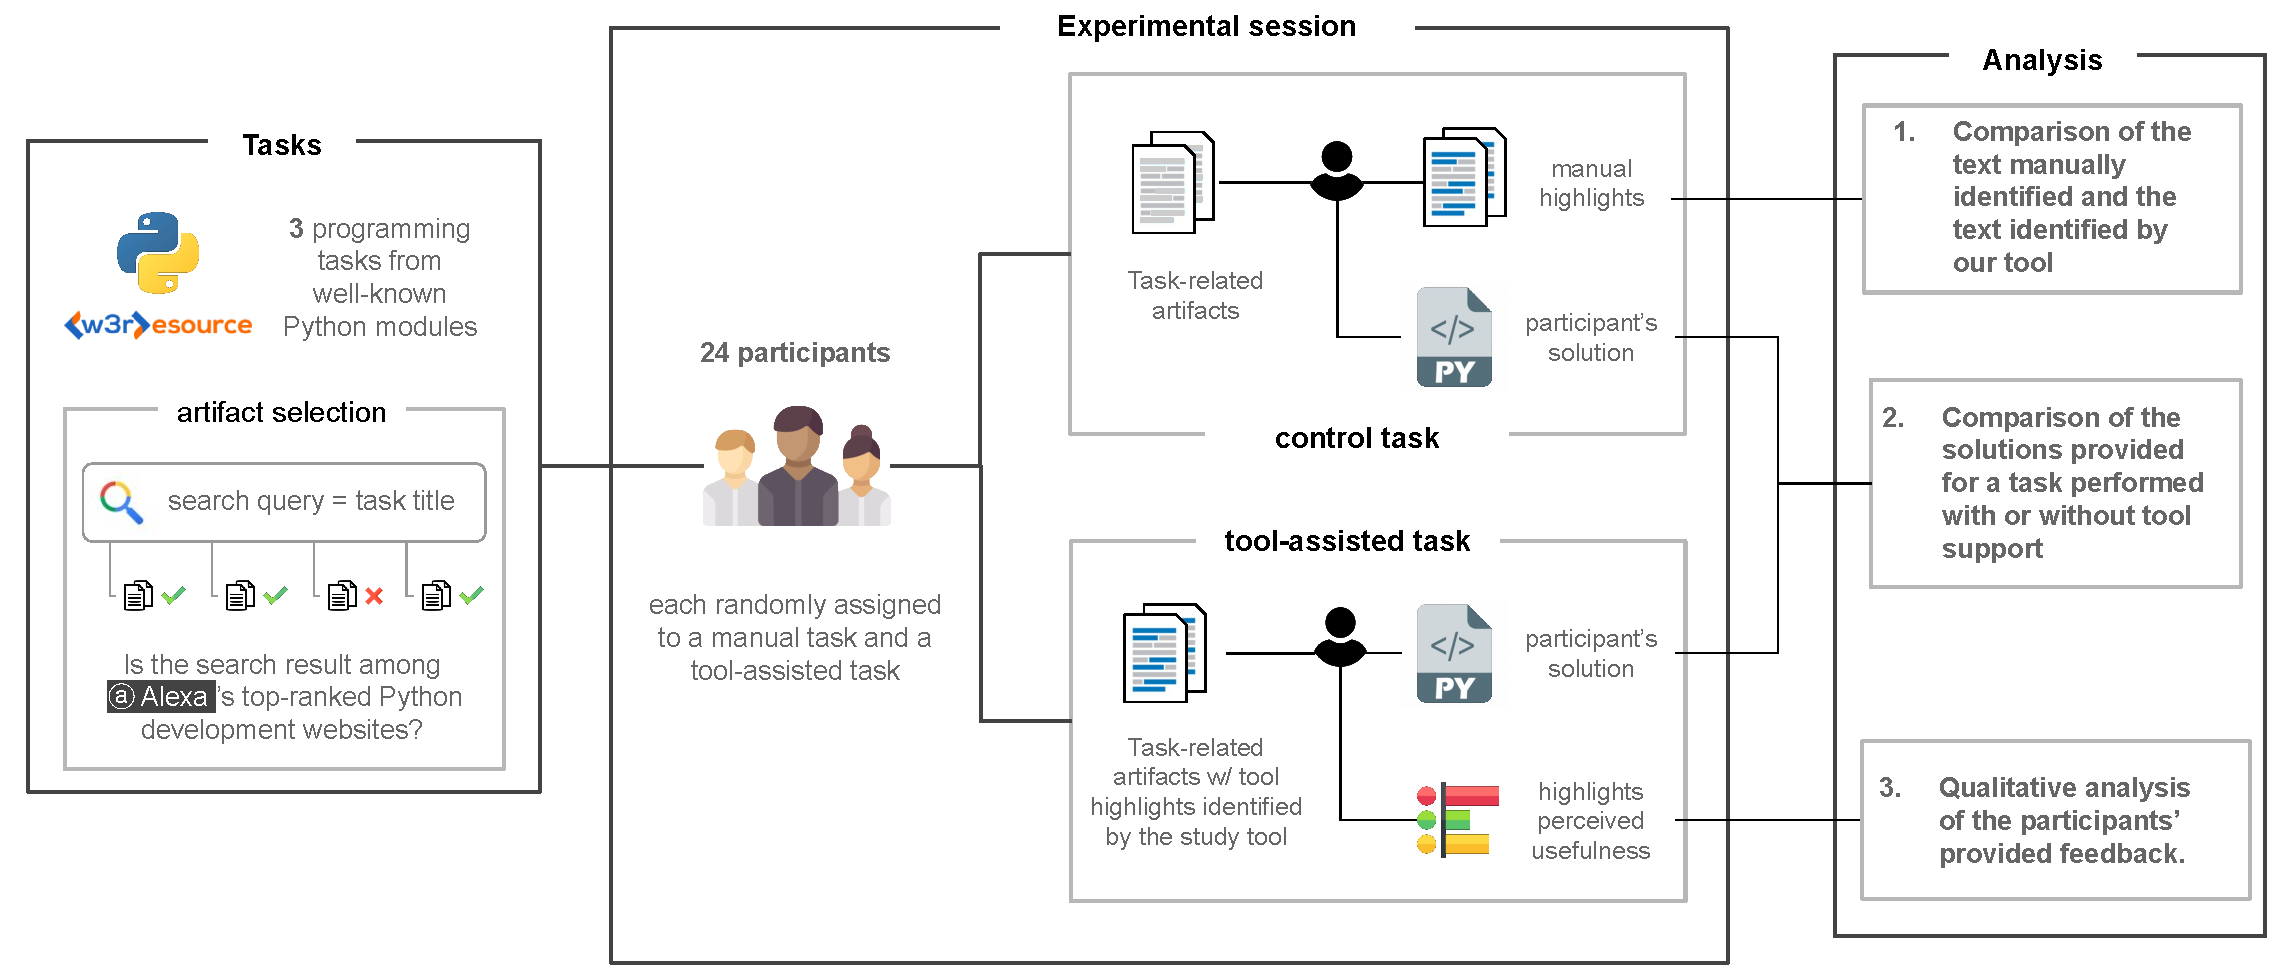
\includegraphics[width=1.05\textwidth]{cp6/tool-experiment-pipeline.pdf}
\caption{Summary of experimental procedures}
\label{fig:tool-experiment-procedures}
\end{figure}





We detail experimental procedures and results in the reminder of this chapter.





 
% On their own time and computer\footnote{Literature define this as an \textit{offline} experiment~\cite{wohlin2012, DeLucia2012}}, we expect that a participant in out experiment attempts two tasks. 
% In a first task, i.e., \textit{manual task}, a participant indicates 
% what text they deem relevant to the task at hand while 
% they consult a 
% In a second task, i.e., \textit{tool-assisted task},
% a participant should write their solution consulting a similar list of curated artifacts, but
% assisted by a tool that highlights the text identified as potentially relevant to their task; for this task, we also gathered feedback on the usefulness of the highlights shown.

 

% With this experiment we evaluate different factors that can help us answer whether 
% a tool embedding a semantic-based technique helps developers complete a software task. 